\documentclass{beamer}




\usepackage[T1,T2A]{fontenc}
\usepackage[utf8]{inputenc}

\usepackage{graphicx}
\usepackage{blindtext}
\usepackage{ mathrsfs }
\usepackage[russian,english]{babel}
\usepackage{listings}
\lstset{language=Pascal} 


\author{Деркач Максим Юрьевич}
\title{Криптографические протоколы}
\subtitle{Лекция 5 \\ Протоколы сильной аутентификации }
\setbeamercolor{frametitle}{bg=cyan!10}

%\usetheme{lucid}
\begin{document}
	\frame {
		\titlepage
	}
	\frame {
	\frametitle{Ссылки}
	
	\url{https://habr.com/post/154229/}
	\url{https://habr.com/en/company/dataart/blog/262817/}
	
	}
	
	\frame{
		\frametitle{Классификация протоколов сильной аутентификации}
		\begin{itemize}
				\item[*] на основе симметричных алгоритмов шифрования;
				\item[*] на основе асимметричных алгоритмов шифрования;
				\item[*] на основе ЭЦП.	
		\end{itemize}
	}

	\frame{
		\frametitle{Протоколы сильной аутентификации}
		\framesubtitle{На основе симметричных алгоритмов шифрования}
		
		\textbf{ISO/ IEC 9798 - 2}
		\begin{enumerate}
			\item $A -> B: text_2 || E_{K_{AB}}(T_A/N_A || ID_B || text_1)$
			\item $B -> A: text_4 || E_{K_{AB}}(T_B/N_B || ID_A || text_3)$
		\end{enumerate}

		\bigskip

		\begin{enumerate}
			\item $B -> A: R_B || text_1$
			\item $A -> B: text_3 || E_{K_{AB}}(R_B || ID_B || text_2)$
		\end{enumerate}
	
		\bigskip
		
		\begin{enumerate}
			\item $B -> A: R_B || text_1$
			\item $A -> B: text_3 || E_{K_{AB}}(R_A || R_B || ID_B || text_2)$
			\item $B -> A: text_5 || E_{K_{AB}}(R_B || R_A || text_4)$
		\end{enumerate}
		\textbf{Замечание} 
		Длина $ID_B || text_2$ не должна равняться длине $text_4$
		
		
	}
	
	\frame{
		\frametitle{Протоколы сильной аутентификации}
		\framesubtitle{На основе симметричных алгоритмов шифрования}
		
		\textbf{Протокол Ву-Лама (Woo-Lam)}
		\begin{enumerate}
			\item $A -> B: ID_A$
			\item $B -> A: R_B$
			\item $A -> B: E_{K_{AT}}(R_B)$
			\item $B -> T: E_{K_{BT}}(ID_A || E_{K_{AT}}(R_B))$
			\item $T -> B: E_{K_{BT}}(R_B)$
		\end{enumerate}
	}

	\frame{
		\frametitle{Протоколы сильной аутентификации}
		\framesubtitle{На основе симметричных алгоритмов шифрования}
		
		\textbf{Атака параллельного сеанса}
		\begin{enumerate}
			\item[1]  $I(A) -> B: ID_A$
			\item[1'] $I -> B: ID_I$
			
			\item[2]  $B -> I(A): R_B$
			\item[2'] $B -> I: R_B^*$
			
			
			\item[3]  $I(A) -> B: E_{K_{IT}}(R_B)$
			\item[3'] $I -> B: E_{K_{IT}}(R_B)$
			
			
			\item[4]  $B -> T: E_{K_{BT}}(ID_A || E_{K_{IT}}(R_B))$
			\item[4'] $B -> T: E_{K_{BT}}(ID_I || E_{K_{IT}}(R_B))$
			
			
			\item[5]  $T -> B: E_{K_{BT}}(MYCOP)$
			\item[5'] $T -> B: E_{K_{BT}}(R_B)$
		\end{enumerate}	
	}
	
		\frame{
		\frametitle{Протоколы сильной аутентификации}
		\framesubtitle{На основе симметричных алгоритмов шифрования}
		
		\textbf{Протокол Отвея-Риса*}
		\begin{enumerate}
			\item $A -> B: ID_A || ID_B || K_{AT}(ID_A || ID_B || N_A || R_A) || N_A$
			\item $B -> T: ID_A || ID_B || K_{AT}(ID_A || ID_B || N_A || R_A) ||$\\ 
			 \quad \quad \quad  \quad \ $K_{BT}(ID_A || ID_B || N_A || R_B) || N_A$
			\item $T -> B: E_{K_{AT}}(K || R_A) || E_{K_{BT}}( K ||R_B) || N_A$
			\item $B -> A: E_{K_{AT}}(K || R_A) || E_{K}( R_A ||R_B) || N_A$
			\item $A -> B: E_{K}(R_B)$
		\end{enumerate}
	
		\bigskip
	
		\textbf{Протокол с использованием хэш-функции}
		\begin{enumerate}
			\item $B -> A: R_B$
			\item $A -> B: R_A || H_{K_{AB}}(R_A || R_B || ID_B)$
			\item $B -> A: H_{K_{AB}}(R_B || R_A || ID_A)$
		\end{enumerate}
	}
	
	\frame{
		\frametitle{Протоколы сильной аутентификации}
		\framesubtitle{На основе асимметричных алгоритмов шифрования}
		
		\textbf{С использованием хэш-функции*}
		\begin{enumerate}
			\item  $B -> A: h(R_B) || ID_B || E_{K_A}^{pub}(R_B || ID_B)$
			\item  $A -> B: R_B$
		\end{enumerate}	
	
		\bigskip
		
		
		\textbf{NSPK}
		\begin{enumerate}
			\item  $A -> B: E_{K_B^{pub}}(R_A || ID_A)$
			\item  $B -> A: E_{K_A^{pub}}(R_A || R_B)$
			\item  $A -> B: E_{K_B^{pub}}(R_B)$
		\end{enumerate}	
	}


	\frame{
		\frametitle{Протоколы сильной аутентификации}
		\framesubtitle{На основе асимметричных алгоритмов шифрования}
		
		\textbf{Атака параллельного сеанса}
		\textbf{NSPK}
		\begin{enumerate}
			\item[1]   $A -> I: E_{K_I^{pub}}(R_A || ID_A)$
			\item[1']  $I(A) -> B: E_{K_B^{pub}}(R_A || ID_A)$
			
			\item[2]   $B -> I(A): E_{K_A^{pub}}(R_A || R_B)$
			\item[2']  $I -> A: E_{K_A^{pub}}(R_A || R_B)$
			
			\item[3]   $A -> I: E_{K_I^{pub}}(R_B)$
			\item[3']  $I(A) -> B: E_{K_B^{pub}}(R_B)$
			
		\end{enumerate}	
	
	}

\frame{
	\frametitle{Протоколы сильной аутентификации}
	\framesubtitle{На основе асимметричных алгоритмов шифрования}
	
	\textbf{Защита}
	\begin{itemize}
		
		\item
		\begin{enumerate}
			\item[2]  $B -> A: E_{K_A^{pub}}(R_A || R_B  || ID_B)$
		\end{enumerate}	
		\item
		\begin{enumerate}
			\item[3]  $A -> B: E_{K_{h(R_B)}}(ID_B)$
		\end{enumerate}	
		
	\end{itemize}
}
	
	\frame{
		\frametitle{Протоколы сильной аутентификации}
		\framesubtitle{С использованием ЭЦП}
		
		
		\textbf{Mech 1.}
		\begin{enumerate}
			\item  $A -> B: cert_A || T_A / N_A || ID_B || sign_A(T_A/N_A || ID_B || text1) $
			\item  $B -> A: cert_B || T_B / N_B || ID_A || sign_B(T_B/N_B || ID_A || text3) $
		\end{enumerate}	
		
		\bigskip
		

		\textbf{Mech 2.}
		\begin{enumerate}
			\item  $B -> A: R_B$
			\item  $A -> B: cert_A || R_A || R_B || ID_B || sign_A(R_A || R_B || ID_B)$
			\item  $B -> A: cert_B || R_B || R_A || ID_A || sign_B(R_B || R_A || ID_A)$
		\end{enumerate}	

	}

	\frame{
		\frametitle{Протоколы сильной аутентификации}
		\framesubtitle{С использованием ЭЦП}
	
		
		
		\textbf{Атака}
		\begin{enumerate}
			\item  $I(B) -> A: R_B$
			\item  $A -> I(B): cert_A || R_A || R_B || ID_B || sign_A(R_A || R_B || ID_B)$
			
			\item[1']  $I(A) -> B: R_A$
			\item[2']  $B -> I(A): cert_B || R_B' || R_A || ID_A || sign_B(R_B' || R_A || ID_A )$
			
			
			\item  $I(B) -> A: cert_B || R_B' || R_A || ID_A || sign_B(R_B' || R_A || ID_A )$
		\end{enumerate}	
	}


	\frame{
		\frametitle{Протоколы сильной аутентификации}
		\framesubtitle{Примеры[Аутентификация по сертификатам]}
		
		Сертификат представляет собой набор атрибутов, идентифицирующих владельца, подписанный certificate authority (CA). 
		\bigskip
		
		CA выступает в роли посредника, который гарантирует подлинность сертификатов.
		\bigskip
		
		Также сертификат криптографически связан с закрытым ключом, который хранится у владельца сертификата и позволяет однозначно подтвердить факт владения сертификатом.

		
	}

	\frame{
		\frametitle{Протоколы сильной аутентификации}
		\framesubtitle{Примеры[Аутентификация по сертификатам]}
		
		В веб-приложениях традиционно используют сертификаты стандарта X.509. Аутентификация с помощью X.509-сертификата происходит в момент соединения с сервером и является частью протокола SSL/TLS.
		
		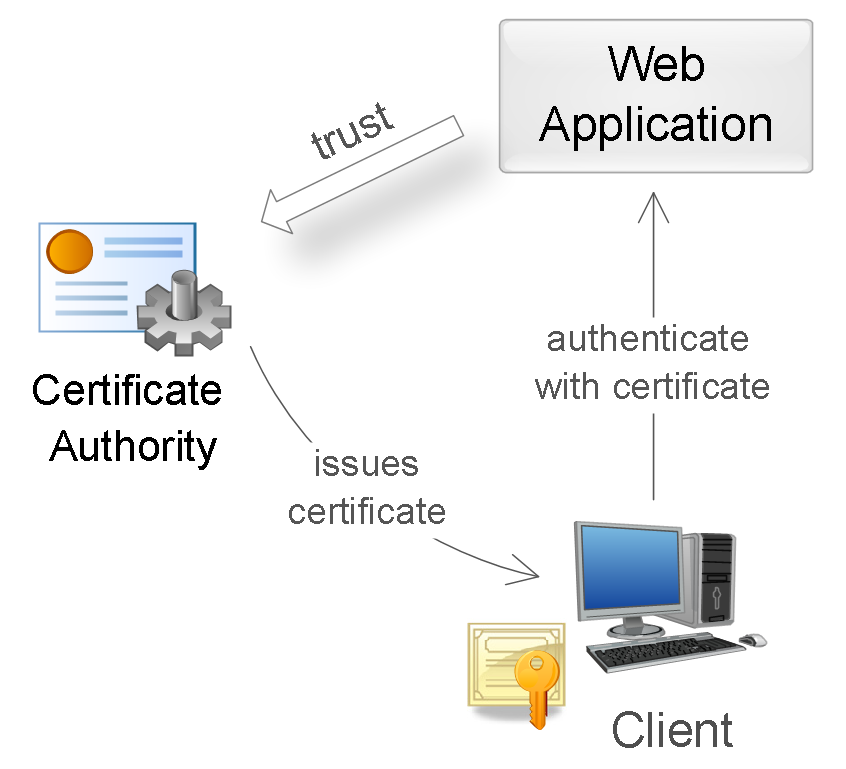
\includegraphics[width=0.6\linewidth]{cert.png}
		
		
	}

	\frame{
		\frametitle{Протоколы сильной аутентификации}
		\framesubtitle{Примеры[Аутентификация по сертификатам]}
	

		Во время аутентификации сервер выполняет проверку сертификата на основании следующих правил:
		
		\bigskip
		\begin{enumerate}
			\item Сертификат должен быть подписан доверенным certification authority (проверка цепочки сертификатов).
			\item Сертификат должен быть действительным на текущую дату (проверка срока действия).
			\item Сертификат не должен быть отозван соответствующим CA (проверка списков исключения).
		\end{enumerate}
	}

	\frame{
		\frametitle{Протоколы сильной аутентификации}
		\framesubtitle{Примеры[JWT]}
		
		\textbf{JSON Web Token (JWT)} — содержит три блока, разделенных точками: заголовок, набор полей (claims) и подпись. 
		\bigskip 
		
		Первые два блока представлены в JSON-формате и дополнительно закодированы в формат base64. 
		\bigskip
		
		Набор полей содержит произвольные пары имя/значения, притом стандарт JWT определяет несколько зарезервированных имен (iss, aud, exp и другие). 
		\bigskip
		
		Подпись может генерироваться при помощи и симметричных алгоритмов шифрования, и асимметричных.
		
		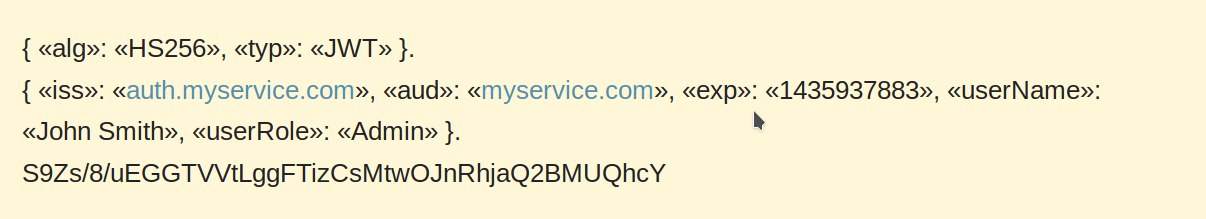
\includegraphics[width=0.8\linewidth]{s.png}
		
	}

	\frame {
	\begin{figure}
		
\includegraphics[width=0.8\linewidth]{meme.png}
	
	\end{figure}
	}

\end{document}